\documentclass[10pt, onecolumn]{scrartcl}
\usepackage{amsmath, graphicx}
\usepackage{xcolor}
\usepackage[top=1in, bottom=1in, left=1in, right=1in, includefoot]{geometry}
\usepackage{fancyvrb}
\usepackage{siunitx}
\usepackage[formats]{listings}
\usepackage[unicode=true]{hyperref}
\usepackage{enumitem}


\lstdefinelanguage{ucf}{
  sensitive=false,
  alsoletter={.},
  morekeywords={NET,LOC},
  morecomment=[l]{\#},
  morestring=[b]"
}


\lstdefineformat{Vlog}{~=\( \sim \),^=\(^\wedge\)}

\lstset{ %
  basicstyle=\ttfamily,        % the size of the fonts that are used for the code
  	format=Vlog,
  breaklines=false,                 % sets automatic line breaking
  language=Verilog,
  commentstyle=\color{red},    % comment style
  frame=single,                    % adds a frame around the code
  keepspaces=true,                 % keeps spaces in text, useful for keeping indentation of code (possibly needs columns=flexible)
  keywordstyle=\color{blue},       % keyword style
  morekeywords={*,...},            % if you want to add more keywords to the set
  rulecolor=\color{black},         % if not set, the frame-color may be changed on line-breaks within not-black text (e.g. comments (green here))
  showspaces=false,                % show spaces everywhere adding particular underscores; it overrides 'showstringspaces'
  tabsize=7,                       % sets default tabsize to 2 spaces
}

\usepackage{tikz}
\usepackage[american]{circuitikz}
\usetikzlibrary{calc,positioning,arrows,shapes.geometric}

\tikzset{
  multiplexer/.style={
    draw,
    trapezium,
    shape border uses incircle, 
    shape border rotate=270,
    minimum size=18pt
  }  
}


\ctikzset{bipoles/not port/circle width=0.4}

\begin{document}
%%%%%%%%%%%%%%%%%%%%%%%%%%%%%%%%%%%%%%%%%%%%%%%%%%%%%%%
\title{ECE 2700 Lab 5\\ Sequential Circuits}%\& Finite State Machines}
\subtitle{Due at the end of your registered lab session (130 points)}
\date{}
\maketitle

\vspace{-0.5in}

\begin{center}
{\Large Objectives} \\
\vspace{0.1cm}
\begin{itemize}
	\item Theory Objectives:
	\begin{itemize}
		\item R/S and D latches
		\item Master-slave flip-flops: R/S, D, J/K and T
		\item Basic register design with \texttt{set} and \texttt{clear} (i.e.\ \texttt{reset}) capability.
		\item Register architectures for implementing shift-register and binary counter modules.
	\end{itemize}

	\item Verilog Syntax and Design Objectives
	\begin{itemize}
		\item Verilog description of level-sensitive transparent latches vs edge-sensitive flip-flops.
		\item Inferred latches and flip-flops.
		\item Synthesizable Structural or Behavioral designs, vs Data Flow modeling techniques.
	\end{itemize}
\end{itemize}

\end{center}


\section{Pre-Lab Exercises}

\begin{enumerate}
	\item A standard RS latch is shown below. Assume each gate has a delay of one ``time unit'' (\texttt{tu} for short). A grid of time units is shown in the diagram below, along with the $S$ and $R$ signals at each time. The initial values of $Q$ and $Q^\prime$ are shown. Complete the timing diagram for signals $Q$ and $Q^\prime$, and explain what will happen at the end after $S=R=1$.
	\begin{center}
		\ctikzset{bipoles/not port/circle width=0.4}
\ctikzset{tripoles/american nand port/circle width=0.4}
\ctikzset{tripoles/american nor port/circle width=0.4}
\ctikzset{tripoles/american nor port/input height=0.6}
\ctikzset{tripoles/american nor port/input skip=0.18}
\ctikzset{tripoles/american xnor port/circle width=0.4}
\ctikzset{tripoles/american and port/port width=0.4}
\ctikzset{tripoles/american and port/input height=0.6}
\ctikzset{tripoles/american or port/port width=0.5}
\ctikzset{tripoles/american or port/input skip=0.2}
\ctikzset{tripoles/american or port/aaa=0.4}
\ctikzset{tripoles/american or port/bbb=0.2}
\ctikzset{tripoles/american or port/ccc=0.7}
\ctikzset{tripoles/american xor port/port width=0.5}
\ctikzset{tripoles/american xor port/input skip=0.15}
\ctikzset{tripoles/american xor port/aaa=0.4}
\ctikzset{tripoles/american xor port/bbb=0.2}
\ctikzset{tripoles/american xor port/ccc=0.7}
\ctikzset{tripoles/american xnor port/port width=0.75}
\ctikzset{tripoles/american xnor port/input skip=0.2}
\ctikzset{tripoles/american xnor port/aaa=0.5}
\ctikzset{tripoles/american xnor port/bbb=0.4}
\ctikzset{tripoles/american xnor port/ccc=0.4}
\ctikzset{tripoles/pmos/gate width=0.5}
\ctikzset{tripoles/pmos/base width=0.4}
\ctikzset{nodes width=0.075}
\begin{tikzpicture}
  \node[nor port] at (0,0) (nor1) {};
  \node[nor port] at (0,-2) (nor2) {};

  \draw (nor1.out) to[short,*-] ++(0,-0.25) coordinate (qa) (nor2.in 1) -- ++(0,0.25) -- (qa);
  \draw (nor2.out) to[short,*-] ++(0,0.25) coordinate (qb) (nor1.in 2) -- ++(0,-0.25) -- (qb);
  \draw (nor1.out) -- ++(0.5,0) node[anchor=west] {$Q^\prime$};
  \draw (nor2.out) -- ++(0.5,0) node[anchor=west] {$Q$};
  \draw (nor1.in 1) -- ++(-0.5,0) node[anchor=east] {$S$};
  \draw (nor2.in 2) -- ++(-0.5,0) node[anchor=east] {$R$};

  \node[anchor=north west] at (2,1) {\begin{minipage}{10cm}
\begin{tikztimingtable}[%
 timing/dslope =0.1 , timing/.style={x=1ex ,y=6ex }, x =2 ex ,
 timing/rowdist =8ex ,
 timing/name/.style ={ font =\sffamily \scriptsize },
% timing/nodes/advanced,
 ]
  %%%%%%%%%%%%%%%%%%%%%%%%%%%%%%%%%%%%%
%
  {$S$} & 6.0 L 6H 20L 6H 18L  \\
  {$R$} & 18.0 L 6H 8L 6H 18L \\
  {$Q$} & 2L ;[ dotted ] 2L;\\
  {$Q^\prime$} & 2H ;[ dotted ] 2H;\\
%
  %%%%%%%%%%%%%%%%%%%%%%%%%%%%%%%%%%%%%
  \extracode
  \begin{pgfonlayer}{background}
    \begin{scope}[gray,semitransparent,semithick]
      \horlines {}
      \foreach \x in {0,1,...,28} {
        \draw (\x,4) -- (\x,-15);
      };
    \end{scope}
  \end{pgfonlayer}
\end{tikztimingtable}
  \end{minipage}
  };
\end{tikzpicture}
	\end{center}
	\item Repeat exercise 1 under the assumption that the second (bottom) NOR gate has a delay of 2\texttt{tu}. How will that affect the events at the end?
	\begin{center}
		\ctikzset{bipoles/not port/circle width=0.4}
\ctikzset{tripoles/american nand port/circle width=0.4}
\ctikzset{tripoles/american nor port/circle width=0.4}
\ctikzset{tripoles/american nor port/input height=0.6}
\ctikzset{tripoles/american nor port/input skip=0.18}
\ctikzset{tripoles/american xnor port/circle width=0.4}
\ctikzset{tripoles/american and port/port width=0.4}
\ctikzset{tripoles/american and port/input height=0.6}
\ctikzset{tripoles/american or port/port width=0.5}
\ctikzset{tripoles/american or port/input skip=0.2}
\ctikzset{tripoles/american or port/aaa=0.4}
\ctikzset{tripoles/american or port/bbb=0.2}
\ctikzset{tripoles/american or port/ccc=0.7}
\ctikzset{tripoles/american xor port/port width=0.5}
\ctikzset{tripoles/american xor port/input skip=0.15}
\ctikzset{tripoles/american xor port/aaa=0.4}
\ctikzset{tripoles/american xor port/bbb=0.2}
\ctikzset{tripoles/american xor port/ccc=0.7}
\ctikzset{tripoles/american xnor port/port width=0.75}
\ctikzset{tripoles/american xnor port/input skip=0.2}
\ctikzset{tripoles/american xnor port/aaa=0.5}
\ctikzset{tripoles/american xnor port/bbb=0.4}
\ctikzset{tripoles/american xnor port/ccc=0.4}
\ctikzset{tripoles/pmos/gate width=0.5}
\ctikzset{tripoles/pmos/base width=0.4}
\ctikzset{nodes width=0.075}
\begin{tikzpicture}
  \node[nor port] at (0,0) (nor1) {};
  \node[nor port] at (0,-2) (nor2) {};

  \draw (nor1.out) to[short,*-] ++(0,-0.25) coordinate (qa) (nor2.in 1) -- ++(0,0.25) -- (qa);
  \draw (nor2.out) to[short,*-] ++(0,0.25) coordinate (qb) (nor1.in 2) -- ++(0,-0.25) -- (qb);
  \draw (nor1.out) -- ++(0.5,0) node[anchor=west] {$Q^\prime$};
  \draw (nor2.out) -- ++(0.5,0) node[anchor=west] {$Q$};
  \draw (nor1.in 1) -- ++(-0.5,0) node[anchor=east] {$S$};
  \draw (nor2.in 2) -- ++(-0.5,0) node[anchor=east] {$R$};

  \node[anchor=north west] at (2,1) {\begin{minipage}{10cm}
\begin{tikztimingtable}[%
 timing/dslope =0.1 , timing/.style={x=1ex ,y=6ex }, x =2 ex ,
 timing/rowdist =8ex ,
 timing/name/.style ={ font =\sffamily \scriptsize },
% timing/nodes/advanced,
 ]
  %%%%%%%%%%%%%%%%%%%%%%%%%%%%%%%%%%%%%
%
  {$S$} & 6.0 L 6H 20L 6H 18L  \\
  {$R$} & 18.0 L 6H 8L 6H 18L \\
  {$Q$} & 2L ;[ dotted ] 2L;\\
  {$Q^\prime$} & 2H ;[ dotted ] 2H;\\
%
  %%%%%%%%%%%%%%%%%%%%%%%%%%%%%%%%%%%%%
  \extracode
  \begin{pgfonlayer}{background}
    \begin{scope}[gray,semitransparent,semithick]
      \horlines {}
      \foreach \x in {0,1,...,28} {
        \draw (\x,4) -- (\x,-15);
      };
    \end{scope}
  \end{pgfonlayer}
\end{tikztimingtable}
  \end{minipage}
  };
\end{tikzpicture}
	\end{center}
	\item A clock-enabled RS latch is shown below, along with some signal timings. Assuming effectively zero gate delay, predict the signal outputs $Q$ and $Q^\prime$.
	\begin{center}
		\ctikzset{bipoles/not port/circle width=0.4}
\ctikzset{tripoles/american nand port/circle width=0.4}
\ctikzset{tripoles/american nor port/circle width=0.4}
\ctikzset{tripoles/american nor port/input height=0.6}
\ctikzset{tripoles/american nor port/input skip=0.18}
\ctikzset{tripoles/american xnor port/circle width=0.4}
\ctikzset{tripoles/american and port/port width=0.4}
\ctikzset{tripoles/american and port/input height=0.6}
\ctikzset{tripoles/american or port/port width=0.5}
\ctikzset{tripoles/american or port/input skip=0.2}
\ctikzset{tripoles/american or port/aaa=0.4}
\ctikzset{tripoles/american or port/bbb=0.2}
\ctikzset{tripoles/american or port/ccc=0.7}
\ctikzset{tripoles/american xor port/port width=0.5}
\ctikzset{tripoles/american xor port/input skip=0.15}
\ctikzset{tripoles/american xor port/aaa=0.4}
\ctikzset{tripoles/american xor port/bbb=0.2}
\ctikzset{tripoles/american xor port/ccc=0.7}
\ctikzset{tripoles/american xnor port/port width=0.75}
\ctikzset{tripoles/american xnor port/input skip=0.2}
\ctikzset{tripoles/american xnor port/aaa=0.5}
\ctikzset{tripoles/american xnor port/bbb=0.4}
\ctikzset{tripoles/american xnor port/ccc=0.4}
\ctikzset{tripoles/pmos/gate width=0.5}
\ctikzset{tripoles/pmos/base width=0.4}
\ctikzset{nodes width=0.075}
\begin{tikzpicture}
  \node[nor port] at (0,0) (nor1) {};
  \node[nor port] at (0,-2) (nor2) {};

  \draw (nor1.out) to[short,*-] ++(0,-0.25) coordinate (qa) (nor2.in 1) -- ++(0,0.25) -- (qa);
  \draw (nor2.out) to[short,*-] ++(0,0.25) coordinate (qb) (nor1.in 2) -- ++(0,-0.25) -- (qb);
  \draw (nor1.out) -- ++(0.5,0) node[anchor=west] {$Q^\prime$};
  \draw (nor2.out) -- ++(0.5,0) node[anchor=west] {$Q$};

  \draw (nor1.in 1) -- ++(-0.5,0) node[and port, anchor=out] (and1) {};
  \draw (nor2.in 2) -- ++(-0.5,0) node[and port, anchor=out] (and2) {};
  \draw (and1.in 2) -- (and2.in 1);
  \draw ($(and1.in 2)!0.5!(and2.in 1)$) to[short,*-] ++(-0.5,0) node[anchor=east] {\texttt{clk}};
  \draw (and1.in 1) -- ++(-0.5,0) node[anchor=east] {$S$};
  \draw (and2.in 2) -- ++(-0.5,0) node[anchor=east] {$R$};


  \node[anchor=north west] at (2,1) {\begin{minipage}{10cm}
\begin{tikztimingtable}[%
 timing/dslope =0.1 , timing/.style={x=1ex ,y=6ex }, x =2 ex ,
 timing/rowdist =8ex ,
 timing/name/.style ={ font =\sffamily \scriptsize },
% timing/nodes/advanced,
 ]
  %%%%%%%%%%%%%%%%%%%%%%%%%%%%%%%%%%%%%
%
  {$S$} & 4L 10{4C}  \\
  {$R$} & 8.0L 9{4C} \\
  {\texttt{clk}} & 1.75L 2H 2L 4H 2L 2H 4L 2H 2L 4H 2L 2H 4L 2H 2L 4H 2L \\
  {$Q$} & 2L ;[ dotted ] 2L;\\
  {$Q^\prime$} & 2H ;[ dotted ] 2H;\\
%
  %%%%%%%%%%%%%%%%%%%%%%%%%%%%%%%%%%%%%
  \extracode
  \begin{pgfonlayer}{background}
    \begin{scope}[gray,semitransparent,semithick]
      \horlines {}
      \foreach \x in {0,1,...,22} {
        \draw (\x,4) -- (\x,-20);
      };
    \end{scope}
  \end{pgfonlayer}
\end{tikztimingtable}
  \end{minipage}
  };

\end{tikzpicture}
	\end{center}
	\item An edge-sensitive master/slave RS flip-flop is shown below, along with some signal timings. Assuming effectively zero gate delay, predict the signal outputs $Q$ and $Q^\prime$.
	\begin{center}
		\ctikzset{bipoles/not port/circle width=0.4}
\ctikzset{tripoles/american nand port/circle width=0.4}
\ctikzset{tripoles/american nor port/circle width=0.4}
\ctikzset{tripoles/american nor port/input height=0.6}
\ctikzset{tripoles/american nor port/input skip=0.18}
\ctikzset{tripoles/american xnor port/circle width=0.4}
\ctikzset{tripoles/american and port/port width=0.4}
\ctikzset{tripoles/american and port/input height=0.6}
\ctikzset{tripoles/american or port/port width=0.5}
\ctikzset{tripoles/american or port/input skip=0.2}
\ctikzset{tripoles/american or port/aaa=0.4}
\ctikzset{tripoles/american or port/bbb=0.2}
\ctikzset{tripoles/american or port/ccc=0.7}
\ctikzset{tripoles/american xor port/port width=0.5}
\ctikzset{tripoles/american xor port/input skip=0.15}
\ctikzset{tripoles/american xor port/aaa=0.4}
\ctikzset{tripoles/american xor port/bbb=0.2}
\ctikzset{tripoles/american xor port/ccc=0.7}
\ctikzset{tripoles/american xnor port/port width=0.75}
\ctikzset{tripoles/american xnor port/input skip=0.2}
\ctikzset{tripoles/american xnor port/aaa=0.5}
\ctikzset{tripoles/american xnor port/bbb=0.4}
\ctikzset{tripoles/american xnor port/ccc=0.4}
\ctikzset{tripoles/pmos/gate width=0.5}
\ctikzset{tripoles/pmos/base width=0.4}
\ctikzset{nodes width=0.075}
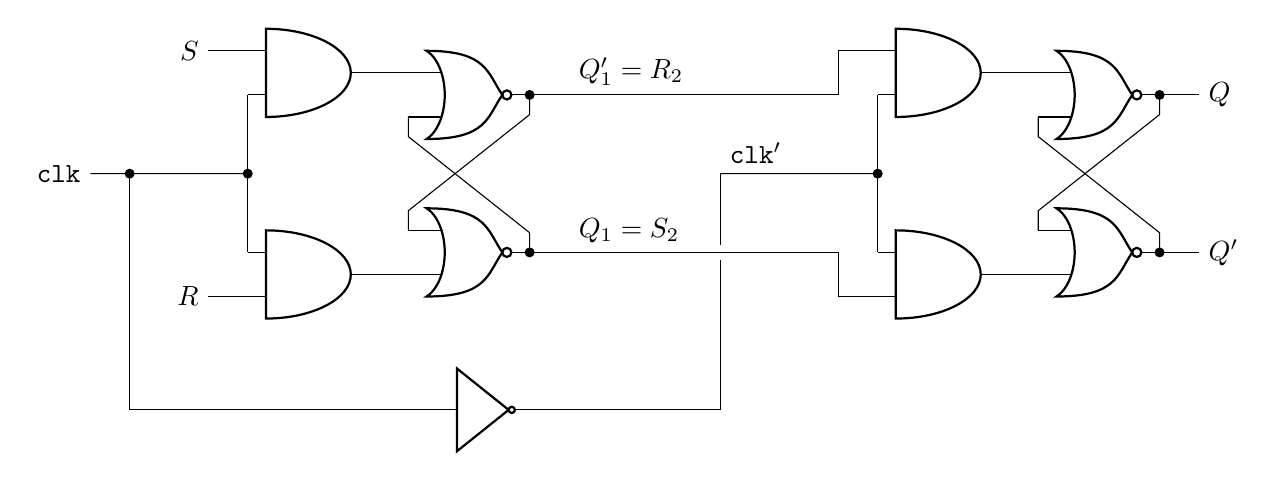
\begin{tikzpicture}
  \node[nor port] at (0,0) (nor1) {};
  \node[nor port] at (0,-2) (nor2) {};

  \draw (nor1.out) to[short,*-] ++(0,-0.25) coordinate (qa) (nor2.in 1) -- ++(0,0.25) -- (qa);
  \draw (nor2.out) to[short,*-] ++(0,0.25) coordinate (qb) (nor1.in 2) -- ++(0,-0.25) -- (qb);
  \draw (nor1.out) -- ++(0.5,0) node[anchor=south west] {$Q_1^\prime=R_2$};
  \draw (nor2.out) -- ++(0.5,0) node[anchor=south west] {$Q_1=S_2$};

  \draw (nor1.in 1) -- ++(-0.5,0) node[and port, anchor=out] (and1) {};
  \draw (nor2.in 2) -- ++(-0.5,0) node[and port, anchor=out] (and2) {};
  \draw (and1.in 2) -- (and2.in 1);
  \draw ($(and1.in 2)!0.5!(and2.in 1)$) coordinate (clk) to[short,*-] ++(-2,0) node[anchor=east] (clkl) {\texttt{clk}};
  \draw (and1.in 1) -- ++(-0.5,0) node[anchor=east] {$S$};
  \draw (and2.in 2) -- ++(-0.5,0) node[anchor=east] {$R$};

  \node[nor port] at (8,0) (nor3) {};
  \node[nor port] at (8,-2) (nor4) {};

  \draw (nor3.out) to[short,*-] ++(0,-0.25) coordinate (qc) (nor4.in 1) -- ++(0,0.25) -- (qc);
  \draw (nor4.out) to[short,*-] ++(0,0.25) coordinate (qd) (nor3.in 2) -- ++(0,-0.25) -- (qd);
  \draw (nor3.out) -- ++(0.5,0) node[anchor=west] {$Q$};
  \draw (nor4.out) -- ++(0.5,0) node[anchor=west] {$Q^\prime$};

  \draw (nor3.in 1) -- ++(-0.5,0) node[and port, anchor=out] (and3) {};
  \draw (nor4.in 2) -- ++(-0.5,0) node[and port, anchor=out] (and4) {};
  \draw (and3.in 2) -- (and4.in 1);
  \draw ($(and3.in 2)!0.5!(and4.in 1)$) to[short,*-] ++(-2,0) coordinate (clkb);
  \node[anchor=south west] at (clkb) {\texttt{clk}$^\prime$};

  \draw (and3.in 1) -- ++(-0.5,0) coordinate (sb) -- (sb |- nor1.out) -- (nor1.out);
  \draw (and4.in 2) -- ++(-0.5,0) coordinate (rb) -- (rb |- nor2.out) -- (nor2.out);

  \draw (clk) ++(-1.5,0) to[short,*-] ++(0,-3) coordinate (x) -- ++(4,0) node[not port,anchor=in,scale=0.75] (inv1) {} (inv1.out) -- (inv1.out -| clkb) coordinate (y)
            (y) -- ($(nor2.out -| y)+(0,-0.1)$) ++ (0,0.2) -- (clkb);

\end{tikzpicture}\\
		
		\begin{tikztimingtable}[%
 timing/dslope =0.1 , timing/.style={x=2ex ,y=6ex }, x =4 ex ,
 timing/rowdist =8ex ,
 timing/name/.style ={ font =\sffamily \scriptsize },
% timing/nodes/advanced,
 ]
  %%%%%%%%%%%%%%%%%%%%%%%%%%%%%%%%%%%%%
%
  {$S$} & 4L 10{4C}  \\
  {$R$} & 8.0L 9{4C} \\
  {\texttt{clk}} & 1.75L 2H 2L 4H 2L 2H 4L 2H 2L 4H 2L 2H 4L 2H 2L 4H 2L \\
  {$Q_1$} & 2L ;[ dotted ] 2L;\\
  {$Q_1^\prime$} & 2H ;[ dotted ] 2H;\\
  {$Q$} & 2L ;[ dotted ] 2L;\\
  {$Q^\prime$} & 2H ;[ dotted ] 2H;\\
%
  %%%%%%%%%%%%%%%%%%%%%%%%%%%%%%%%%%%%%
  \extracode
  \begin{pgfonlayer}{background}
    \begin{scope}[gray,semitransparent,semithick]
      \horlines {}
      \foreach \x in {0,1,...,22} {
        \draw (\x,4) -- (\x,-30);
      };
    \end{scope}
  \end{pgfonlayer}
\end{tikztimingtable}
	\end{center}
	
	\item The flip-flop symbol shown below represents the RS flip flop schematic from the previous exercise. Add the necessary additional components to convert it to a D flip flop.\\
	\vspace{2cm}
	\begin{center}
		\begin{tikzpicture}
			\draw (0,0) rectangle (3,-4);
			\node[anchor=west] at (0,-1) (s)  {$S$};
			\node[anchor=west] at (0,-3) (r)  {$R$};
			\node[anchor=north] at (1.5,0) (clk) {\texttt{clk}};
			\node[anchor=east] at (3,-1) (q) {$Q$};
			\node[anchor=east] at (3,-3) (qb) {$Q^\prime$};
			\draw (clk.north) -- ++(0,0.5);
			\draw (q.east) -- ++(0.5,0);
			\draw (qb.east) -- ++(0.5,0);
			\draw (s.west) -- ++(-0.5,0);
			\draw (r.west) -- ++(-0.5,0);
		\end{tikzpicture}\\
		\vspace{2cm}
	\end{center}
	\pagebreak
	\item A J/K flip-flop is an edge-sensitive memory element with two inputs $J$ and $K$, with behavior defined by the truth table shown below.
% 	Recall that the notation $Q^-$ refers to the value of $Q$ immediately preceding the clock edge.%
	%
	\begin{center}
	    \begin{tabular}{cc|l}
	        $J$ & $K$ & $Q(t+1)$\\ \hline 
	        0 & 0 & $Q(t)$ hold state (no change) \\
	        1 & 0 & 1\\
	        0 & 1 & 0\\
	        1 & 1 & $\sim Q(t)$ toggle state
	    \end{tabular}
	\end{center}
	The flip-flop symbol shown below represents the D flip flop you designed in the previous exercise. Add additional components to convert it to a J/K flip flop, then complete the timing diagram below.\\
	\vspace{3cm}
	\begin{center}
		\begin{tikzpicture}
			\draw (0,0) rectangle (3,-4);
			\node[anchor=west] at (0,-1) (d)  {$D$};
			%\node[anchor=west] at (0,-3) (r)  {$R$};
			\node[anchor=north] at (1.5,0) (clk) {\texttt{clk}};
			\node[anchor=east] at (3,-1) (q) {$Q$};
			\node[anchor=east] at (3,-3) (qb) {$Q^\prime$};
			\draw (clk.north) -- ++(0,0.5);
			\draw (q.east) -- ++(0.5,0);
			\draw (qb.east) -- ++(0.5,0);
			\draw (d.west) -- ++(-0.5,0);
		\end{tikzpicture}\\
		\vspace{3cm}
		\begin{tikztimingtable}[%
 timing/dslope =0.1 , timing/.style={x=2ex ,y=6ex }, x =4 ex ,
 timing/rowdist =8ex ,
 timing/name/.style ={ font =\sffamily \scriptsize },
% timing/nodes/advanced,
 ]
  %%%%%%%%%%%%%%%%%%%%%%%%%%%%%%%%%%%%%
%
  {$J$} & 2{4L} 4H 4L 4H 4L 8H 8L \\
  {$K$} & 4L 4H 12L 12H 8L\\
  {\texttt{clk}} & 5L 17{2C} \\
  {$Q$} & 2L ;[ dotted ] 2L;\\
  {$Q^\prime$} & 2H ;[ dotted ] 2H;\\
%
  %%%%%%%%%%%%%%%%%%%%%%%%%%%%%%%%%%%%%
  \extracode
  \begin{pgfonlayer}{background}
    \begin{scope}[gray,semitransparent,semithick]
      \horlines {}
      \foreach \x in {0,1,...,19} {
        \draw (\x,4) ++(0.5,0) -- ++(0,-26);
      };
    \end{scope}
  \end{pgfonlayer}
\end{tikztimingtable}
	\end{center}	
	
	\pagebreak
	\item Modify your D flip flop again to produce a 1-bit register with extra inputs \texttt{rst}, \texttt{shift}, $D$, and $D_0$. $D_0$ is an initial condition (0 or 1) that is applied when rst is HIGH. The D flip flop has the following functions:\\
	\begin{center}
		\begin{tabular}{crl}
			Function Name & Signal & Operation \\
			\hline
			Reset & \texttt{rst} & when \texttt{rst == 1}, $Q$\texttt{ := } $D_0$\\ 
			Shift & \texttt{shift} & when \texttt{rst == 0} and \texttt{shift == 1}, $Q$\texttt{ := } $D$ \\
			Hold & \texttt{$\overline{\text{shift}}$} & when \texttt{rst == 0} and \texttt{shift == 0}, $Q$\texttt{ := } $Q$
		\end{tabular}
	\end{center}
	\vspace{2cm}
	\begin{center}
		\begin{tikzpicture}
			\draw (0,0) rectangle (3,-4);
			\node[anchor=west] at (0,-1) (d)  {$D$};
			%\node[anchor=west] at (0,-3) (r)  {$R$};
			\node[anchor=north] at (1.5,0) (clk) {\texttt{clk}};
			\node[anchor=east] at (3,-1) (q) {$Q$};
			\node[anchor=east] at (3,-3) (qb) {$Q^\prime$};
			\draw (clk.north) -- ++(0,0.5);
			\draw (q.east) -- ++(0.5,0);
			\draw (qb.east) -- ++(0.5,0);
			\draw (d.west) -- ++(-0.5,0);
		\end{tikzpicture}\\
		\vspace{2cm}
	\end{center}	
	
	\item Show how you can interconnect J/K flip-flops to build a three-bit counter with the following functions:
	\begin{center}
		\begin{tabular}{crl}
		Function & Signal & Description \\
		\hline
		Reset & \texttt{rst} & When \texttt{rst==1}, set all flip-flops to zero\\
		Increment & \texttt{incr} & When \texttt{rst==0} and \texttt{incr==1}, increment the binary count by 1.
		\end{tabular}
		
		\vspace{4cm}
		\begin{tikzpicture}[scale=0.75]
			\foreach \x in {0,1,2} {
				\draw ($7*(\x,0)$) coordinate (nw) rectangle ($7*(\x,0) + (3,-4)$) coordinate (se);
				\node[anchor=west] at ($(nw)+(0,-1)$) (s)  {$J$};
				\node[anchor=west] at ($(nw)+(0,-3)$)(r)  {$K$};
				\node[anchor=north] at ($(nw)+(1.5,0)$) (clk) {\texttt{clk}};
				\node[anchor=east] at ($(nw)+(3,-1)$) (q) {$Q$};
				\node[anchor=east] at ($(nw)+(3,-3)$) (qb) {$Q^\prime$};
				\draw (clk.north) -- ++(0,0.5);
				\draw (q.east) -- ++(0.5,0);
				\draw (qb.east) -- ++(0.5,0);
				\draw (s.west) -- ++(-0.5,0);
				\draw (r.west) -- ++(-0.5,0);
			};
		\end{tikzpicture}
	\end{center}
\end{enumerate}
\pagebreak

\section{RS Latch: Data Flow Model}

One of Verilog's many uses is {\em hardware modeling}, which provides realistic simulations that can include things like signal delays and environmental effects. In this step, we will examine a {\em data flow model} (DFM) of a D flip-flop made from RS latches. A data flow model accounts for physical delays as a signal moves from one gate to another. We have to carefully distinguish DFMs from synthesizable designs, since \textbf{we cannot directly synthesize or modify physical gate delays}. Therefore {\em in this section} you will not program this design onto your Basys3 board, you will just complete a simulation analysis. The purpose of a DFM is to gain deeper understanding of physical signal flow, which sometimes helps us discover rare faults, hazards and glitches, or identify opportunities for physical optimization. The DFM is essentially the same analysis that you performed in Pre-Lab Exercises 1--4. 

In Vivado, create a new project called \texttt{DFF\_dataflow}, and then create a new Verilog module called \texttt{latch\_dataflow}. Your code will model the physical structure of the RS latch, with extra logic to implement a D latch:

\begin{lstlisting}
`timescale 1ns / 1ps

module latch_dataflow(
    input d,
    output q,
    input clk
    );


	wire S;
	wire R;
	wire qb;
	
	assign #1 S=~d&clk;
	assign #1 R=d&clk;
	assign #2 qb=~(R|q);
	assign #2 q=~(S|qb);
\end{lstlisting}
Notice that each \texttt{assign} statement includes a \# statement to declare the assignment's delay. The amount of delay is in units specified by the \texttt{timescale} directive, \SI{1}{\nano\second} in this example. This is the essence of a DFM. Up to now, your Verilog models have presumed instantaneous assignments. That's usually sufficient for fully synchronous clocked designs that use flip-flop registers. When using combinational logic with level-sensitive latches, the pattern of delays can sometimes cause unintended side effects, so there are times when we need to take a close look at it. As a reminder, the delay used above only works in simulation, when running synthesis and implementation these delay statements are ignored as there is no way to create such a delay in the actual FPGA.

Next, create a module named \texttt{DFF\_dataflow} and build it from two instances of your \texttt{latch\_dataflow} module:
\begin{lstlisting}
`timescale 1ns / 1ps

module DFF_dataflow(
    input d,
    output q,
    input clk
    );

	wire q1;
	wire clkb = ~clk;
	
	latch_dataflow d1(.d(d),.q(q1),.clk(clk));
	latch_dataflow d2(.d(q1),.q(q),.clk(clkb));
endmodule
\end{lstlisting}

Finally, create a Verilog testbench to simulate the model. In order to reproduce the \texttt{clk} pattern from Pre-Lab Exercises 3--4, we will create a separate ``master clock'' signal called \texttt{mclk} as the driver for the testbench logic. The irregular \texttt{clk} pattern from the Pre-Lab was generated from a three-bit \texttt{count} signal as shown in the code below.

\begin{lstlisting}
`timescale 1ns / 1ps

module DFF_test;

	// Inputs
	reg d;
	reg clk;
	
	// Outputs
	wire q;

	// Other signals:
	reg mclk;
	reg [2:0] count;

	// Instantiate the Unit Under Test (UUT)
	DFF_dataflow uut (
		.clk(clk), 
		.d(d), 
		.q(q)
	);

	initial begin
		// Initialize Inputs
		clk   = 0;
		d     = 0;
		count = 0;
		mclk  = 0;
		clk   = 0;

		#100;
	end
    
    // generate clock, toggle every 10ns
    always #10 mclk=~mclk; 
    
	always @(posedge mclk) begin
		count = count + 1;
		clk   = count[2]^count[0];
		d     = count[1];
	end
endmodule
\end{lstlisting}

After completing your testbench simulate the model. In the ISim window, click to expand the hierarchy view in the scopes pane (the upper left panel). Expand the \texttt{uut} module to see the \texttt{Dlatch\_dataflow} modules beneath it. Click on each of them, and you should notice that their internal signals appear in the objects panel (just to the right of the hierarchy view). Select the \texttt{S}, \texttt{R}, \texttt{q} and \texttt{qb} signals, and drag them into the waveform viewer panel. Do this for both of the \texttt{Dlatch\_dataflow} submodules, then restart the simulation(loop button on the top ribbon). You should see a pattern of signals that looks very similar to your predictions from the Pre-Lab. Carefully compare the ISim signals to your predictions and verify the same pattern of information. Also take note of any differences that appear. Use the cursors to measure the signal delays, and verify that they match the delays specified in your source code.

\section{D Latch: Behavioral Implementation}

Verilog provides a variety of behavioral methods for implementing latches and flip-flop. In fact, \textbf{any incomplete conditional in an \texttt{always} block will be inferred as a latch.} As a simple example, create a new Verilog module called \texttt{dlatch}, defined as follows:

\begin{lstlisting}
module dlatch(
    input d,
    output reg q,
    input clk
    );
    
    // initial block needed for simulation
    // so that the initial state is defined
    initial begin
        q = 0;
    end
    
	always @(clk or d) begin
		if (clk)
			q <= d;
	end

endmodule
\end{lstlisting}
This simple module is sufficient to define the behavior of a clocked D latch. When \texttt{clk} is asserted, the output \texttt{q} is assigned to equal the input \texttt{d}. When \texttt{clk} is low, the output \texttt{q} is held constant regardless of the value of \texttt{d}. Next, create a new Verilog module named \texttt{DFF}, and copy all the code from \texttt{DFF\_dataflow}. Modify the \texttt{DFF} code so that it instantiates \texttt{dlatch} instead of \texttt{latch\_dataflow}. Then create a testbench, and copy over all code from the previous dataflow testbench, edit it so that it tests \texttt{DFF} instead of \texttt{DFF\_dataflow}, and run the simulation. You should see the same pattern of outputs.

Since this behavioral model is fully synthesizable, you may proceed to create an implementation constraint file. To demonstrate your flip-flop, you will connect the \texttt{clk} signal to switch \texttt{SW0} (\textbf{for this exercise, we will NOT use the usual sys\_clock pin}), and the \texttt{d} signal to \texttt{SW1}. In order to drive the clock from a board switch, Xilinx requires disabling the \texttt{CLOCK\_DEDICATED\_ROUTE} parameter as shown in the code below (this is usually not recommended, but we will do it for this one demonstration). Finally route the output \texttt{q} to one of the LEDs. \textbf{NOTE: make sure you have the \texttt{dlatch} as the top module and not \texttt{latch\_dataflow}, the later cannot be synthesized and will cause a critical error saying something about a combinational loop.}

\begin{lstlisting}[language=xdc]
# Switch SW[0]:
set_property PACKAGE_PIN V17 [get_ports {clk}]
set_property IOSTANDARD LVCMOS33 [get_ports {clk}]
set_property CLOCK_DEDICATED_ROUTE FALSE [get_nets clk_IBUF]

# Switch SW[1]:
set_property PACKAGE_PIN V16 [get_ports {d}]
set_property IOSTANDARD LVCMOS33 [get_ports {d}]

# LED 0:
set_property PACKAGE_PIN U16 [get_ports {q}]				
set_property IOSTANDARD LVCMOS33 [get_ports {q}]
\end{lstlisting}

Set \texttt{dlatch} as your top module, then Synthesize, Implement, and Generate the bit file for your design. Program it onto your Basys3 board and demonstrate the transparent latch function. Turn on \texttt{clk} and observe that \texttt{q} responds when you toggle the \texttt{d} switch. Turn off \texttt{clk} and observe that \texttt{q} no longer responds. Demonstrate this to the TA.

Next, set \texttt{DFF} as the top module and repeat the Synthesis, Implementation and programming procedure. Verify that the output \texttt{q} responds to the value that \texttt{d} has {\em at the precise time when the clock switches}, but it is not at all sensitive to \texttt{d} at other times. Demonstrate this result to the TA. \textbf{This is the main difference between ``level sensitivity'' in latches (which respond when \texttt{clk} is high) vs ``edge sensitivity'' in flip-flops (which respond when \texttt{clk} changes value).} Edge sensitivity is essential for reliable synchronous operation in sequential circuits. 

\section{J/K Flip Flop: Structural Implementation}

Now create a new Verilog module called \texttt{JKFF}. Instantiate your \texttt{DFF} module and add any other logic needed to implement the J/K flip-flop you designed in Pre-Lab exercise 6. Simulate your J/K flip-flop using a Verilog testbench based on the test procedure shown below:

\begin{lstlisting}
module Dlatch_test;
	// Inputs
	reg j;
	reg k;
	reg clk;

	// Outputs
	wire q;

	integer idx;
	
	// J/K test patterns (read from right to left)
	wire [11:0] jvals = 8'b0110_1010;
	wire [11:0] kvals = 8'b0111_0001;
	
	// Instantiate the Unit Under Test (UUT)
	JKFF dut (
		.clk(clk), 
		.j(j),
		.k(k),
		.q(q)
	);

	initial begin
		// Initialize Inputs
		j = 0;
		k = 1;
		idx=0;
		clk = 1;

		#100;
	end
        
    // generate clock, toggle every 10ns
    always #10 clk=~clk; 
    
	always @(posedge clk) begin
		// use modulo arithmetic to increment idx from 0 up to 7,
		// then wrap back to 0:
		idx = (idx + 1) % 8; 
		
		j = jvals[idx];
		k = kvals[idx];
	end
endmodule
\end{lstlisting}

Verify that your flip-flop's behavior matches the prediction from your pre-lab exercise, then proceed to Synthesize, Implement and Program your board using \texttt{SW0} as the \texttt{clk}, \texttt{SW1} as \texttt{j}, and \texttt{SW2} as \texttt{k}, and \texttt{LED0} as \texttt{q}. Verify proper function on your Basys3 board and demonstrate it to the TA.


\section{Shift-Register for Rotating LED Display}

Now create a new project called \texttt{rotateLED}, and add the following module sources into the project:
\begin{itemize}
	\item \texttt{dlatch.v}
	\item \texttt{DFF.v}
	\item \texttt{clockdivider.v} (from Lab 2)
\end{itemize}

Now make a new Verilog module called \texttt{Dregister}. Create an instance of your \texttt{DFF} module, along with any other logic required to implement the multi-function register that you designed in Pre-Lab exercise 7. 

Then create a new Verilog module called \texttt{rotateLED.v} to implement a multi-bit shift register module based on the schematic shown below. Three registers are shown; \textbf{your complete design should use eight registers. You should use a generate block to define the register instances and their interconnections.} For better clarity, this schematic uses connection-by-label, with the top-level module signals shown in blue. At every location labeled \textcolor{blue}{\texttt{shift}}, the same \texttt{shift} signal wire should be connected.

\begin{center}
	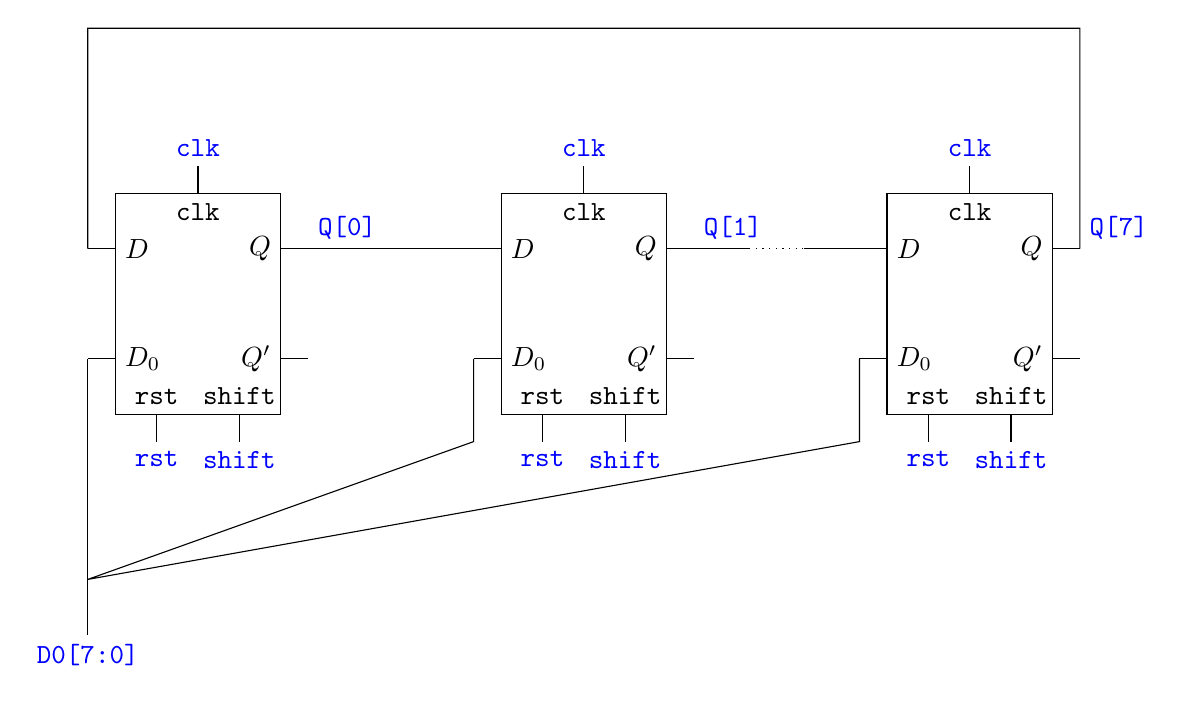
\begin{tikzpicture}[scale=0.7]
			\foreach \x in {0,1,2} {
				\draw ($7*(\x,0)$) coordinate (nw) rectangle ($7*(\x,0) + (3,-4)$) coordinate (se);
				\node[anchor=west] at ($(nw)+(0,-1)$) (d\x)  {$D$};
				\node[anchor=west] at ($(nw)+(0,-3)$)(di\x)  {$D_0$};
				\node[anchor=north] at ($(nw)+(1.5,0)$) (clk\x) {\texttt{clk}};
				\node[anchor=south] at ($(se)-(0.75,0)$) (shift\x) {\texttt{shift}};
				\node[anchor=south] at ($(se)-(2.25,0)$) (rst\x) {\texttt{rst}};
				\node[anchor=east] at ($(nw)+(3,-1)$) (q\x) {$Q$};
				\node[anchor=east] at ($(nw)+(3,-3)$) (qb\x) {$Q^\prime$};
				\draw (clk\x.north) -- ++(0,0.5) coordinate (clkp\x);
				\draw (shift\x.south) -- ++(0,-0.5) coordinate (shiftp\x);
				\draw (rst\x.south) -- ++(0,-0.5) coordinate (rstp\x);
				\draw (q\x.east) -- ++(0.5,0) coordinate (qp\x);
				\draw (qb\x.east) -- ++(0.5,0) coordinate (qbp\x);
				\draw (d\x.west) -- ++(-0.5,0) coordinate (dp\x);
				\draw (di\x.west) -- ++(-0.5,0) coordinate (d0p\x);
				\node[anchor=south,blue] at (clkp\x) {\texttt{clk}};
				\node[anchor=north,blue] at (rstp\x) {\texttt{rst}};
				\node[anchor=north,blue] at (shiftp\x) {\texttt{shift}};
			};
			
			\node[anchor=south west,blue] at (qp0) {\texttt{Q[0]}};
			\node[anchor=south west,blue] at (qp1) {\texttt{Q[1]}};
			\node[anchor=south west,blue] at (qp2) {\texttt{Q[7]}};
			\draw (d0p0) -- ++(0,-4) coordinate (d0_out) -- ++(0,-1) node[anchor=north,blue] {\texttt{D0[7:0]}};
			\draw (d0p1) -- ++(0,-1.5) -- (d0_out) (d0p2) -- ++(0,-1.5)-- (d0_out);
			\draw (qp0) -- (dp1);
			\draw (qp1) -- ++(1,0) coordinate (a);
			\draw (dp2) -- ++(-1,0) coordinate (b);
			\draw[dotted] (a) -- (b);
			\draw (qp2) -- ++(0,4) coordinate (c) -- (c -| dp0) -- (dp0); 
	\end{tikzpicture}
\end{center}

The top-level I/O ports are shown in the table below, along with their intended Basys3 board mappings.

\begin{center}
\begin{tabular}{ccccc}
direction & name & vector & bits & board resource\\
\hline
\texttt{input} & \texttt{mclk} & no & 1 & \texttt{MCLK}\\ 
\texttt{input} & \texttt{shift} & no & 1 & \texttt{BTN0} \\
\texttt{input} & \texttt{rst} & no & 1 & \texttt{BTN1} \\
\texttt{input} & \texttt{D0} & yes & 7:0 & \texttt{SW0} to \texttt{SW7}\\ 
\texttt{output} & \texttt{Q} & yes & 7:0 & \texttt{LD0} to \texttt{LD7}\\ 
\end{tabular}
\end{center}

Use an instance of your \texttt{ClockDivider} module to generate the \texttt{clk} signal for your shift register, so that you can observe sequential events in your implementation. See the next subsection on how to set the \texttt{ClockDivider} divider ratio to be different for implementation vs simulation. We want a divider of 25,000,000 when it's on the physical board but a divider of 1 when simulating. Prepare an Implementation Constraints File for these connections, then Synthesize, Implement and program your design onto the Basys3 board. Use the switches to define a non-zero initial state, then press (and hold) \texttt{BTN1} to reset the shift register. Then, press and hold \texttt{BTN0} to start shifting the pattern. You should see the pattern rotate on the LED display. The process may run very slowly, depending on the divider ratio used in your \texttt{ClockDivider} module. 

\subsection{Different ClockDivider Scaler Values For Simulation and Implementation}
This subsection applies to both the Rotate LED and the Counter designs. Sometimes you may accidentally simulate a design with a very large clock divider value. Since the value is so large, the simulation would have to run for a very long time to see the correct output. It may appear that nothing is working if you only look at a very short time frame. To allow simulation to use a different clock divider value we can add a parameter to the top module like so. This way when the project is built to run on the physical board, it will use 25 million and when the design is simulated, a clock divider value of 1 is used instead. Now, there is no need to keep changing them by hand, depending on if it's for simulation or implementation.

\begin{lstlisting}
module your_top_module #(parameter PRESCALER = 25_000_000)(
    input mclk,
    // add the other needed inputs and outputs here

    );

	wire slow_clk;
	
	ClockDivider  #(.PRESCALER(PRESCALER)) CKD( 
			.clkin(mclk),
			.clkout(slow_clk)
		);
	
	// add other signals, generate statements and modules here
endmodule
\end{lstlisting}

In your testbench, when you instantiate the top module, remember to override the PRESCALER value of 25,000,000 to a value of 1. This way you don't have to simulate for hundreds of milliseconds.

\begin{lstlisting}
your_top_module #(.PRESCALER(1)) DUT(
// add your ports here
    );
\end{lstlisting}
\section{Counter Module}

Lastly, create a new project called \texttt{counter} to implement the J/K flip-flop counter that you designed in Pre-Lab exercise 8. Add the following sources to your project:
\begin{itemize}
	\item \texttt{dlatch.v}
	\item \texttt{DFF.v}
	\item \texttt{JKFF.v}
	\item \texttt{ClockDivider.v}
\end{itemize}

Create a new Verilog source to define the top-level \texttt{counter} module with the following I/O signals:
\begin{center}
\begin{tabular}{ccccc}
direction & name & vector & bits & board resource\\
\hline
\texttt{input} & \texttt{mclk} & no & 1 & \texttt{MCLK}\\ 
\texttt{input} & \texttt{incr} & no & 1 & \texttt{BTN0} \\
\texttt{input} & \texttt{rst} & no & 1 & \texttt{BTN1} \\
\texttt{output} & \texttt{Q} & yes & 7:0 & \texttt{LD0} to \texttt{LD7}\\ 
\end{tabular}
\end{center}

Use a \texttt{generate} loop to instantiate J/K flip-flops and build an eight-bit counter module. Initially prepare the design with no \texttt{ClockDivider} module. Create a Verilog testbench to simulate your model and verify that your counter increments from 0 up to 255 when \texttt{incr} is asserted. Once verified, add the \texttt{ClockDivider} module and then Synthesize, Implement and program the design onto your Basys3 board. The LEDs should clear when you press \texttt{BTN1}, and should show a successive binary sequence when you press and hold \texttt{BTN0}. Demonstrate your design to the TA.

\section{TA Checkoff}

\begin{itemize}
\item (32 points) Complete pre-lab work prior to start of the lab.
\item (12 points) RS latch and DFF dataflow simulation.
\item (12 points) Behavioral D latch and structural DFF simulation and implementation.
\item (20 points) J/K flip-flop simulation and implementation.
\item (24 points) Shift Register design, simulation and implementation.
\item (30 points) Counter design, simulation and implementation.
\end{itemize}

\end{document}